% Author: Victor.I
% Technical architecture review for engineering leads (Beamer + TikZ).
% Compile with pdfLaTeX; requires tikz (standard in TeX Live / Overleaf).

\documentclass[aspectratio=169,11pt]{beamer}

\usetheme{Madrid}
\usecolortheme{default}

\setbeamertemplate{navigation symbols}{}
\setbeamertemplate{footline}[frame number]

\usepackage[T1]{fontenc}
\usepackage[utf8]{inputenc}
\usepackage{lmodern}
\usepackage{microtype}
\usepackage{tikz}
\usetikzlibrary{arrows.meta,positioning,fit,calc,shapes.geometric}

\title[REOS Architecture]{REOS: Technical Architecture \& Delivery Plan}
\subtitle{For engineering and platform leads}
\author{Victor.I}
\date{\today}

\begin{document}

\begin{frame}
  \titlepage
\end{frame}

\begin{frame}{Agenda}
  \tableofcontents
\end{frame}

%------------------------------------------------------------------
\section{Goals and scope}

\begin{frame}{What you are evaluating}
  \small
  \begin{itemize}
    \item \textbf{Platform}: decision-first deal operating system (workflow, CRM, documents, investor pipeline, integrations catalog).
    \item \textbf{Differentiator}: grounded document intelligence + explicit human gates on money, legal, and regulated outreach.
    \item \textbf{Scope of this review}: boundaries, data flows, security posture, evolution to enterprise Azure profile, delivery risk.
  \end{itemize}
  \vspace{0.6em}
  \textbf{Success criteria for the build contract}: observable SLIs, audited automation, clean rollback, no secrets in clients, Postgres-cutover path.
\end{frame}

\begin{frame}{Current repository profile (honest baseline)}
  \small
  \begin{itemize}
    \item \textbf{API}: FastAPI monolith as BFF: auth, domain routes, integration catalog, document ingestion hooks, AI orchestration.
    \item \textbf{Client}: Next.js App Router; bearer sessions against API.
    \item \textbf{Persistence}: SQLAlchemy; default \texttt{sqlite:///./reos.db}; production targets \texttt{REOS\_DATABASE\_URL} (PostgreSQL).
    \item \textbf{AI}: retrieval + LLM provider abstraction (local Ollama vs Azure OpenAI via env).
    \item \textbf{Async}: heavy work today largely in-process; enterprise plan is queue + workers (Service Bus / Functions).
  \end{itemize}
  \vspace{0.5em}
  \textit{Pitch is not ``greenfield slides''---it is an incremental hardening path with defined cutovers.}
\end{frame}

%------------------------------------------------------------------
\section{Vision, audience, and outcomes}

\begin{frame}{Vision: final product}
  \small
  \textbf{North star}: one operating layer where acquisition, diligence, IC preparation, and investor coordination share \textbf{the same transactional truth}, with AI that \textbf{grounds} answers in documents and produces \textbf{auditable} suggestions---not silent autonomy on capital or outbound regulatory touchpoints.

  \vspace{0.6em}
  \textbf{What ``done'' looks like} (contract-level):
  \begin{itemize}\itemsep2pt
    \item Deal workspace is a \textbf{decision surface}: verdict scaffold, gaps, next actions, time-in-stage metrics.
    \item Document path is \textbf{pipeline}: upload $\rightarrow$ parse $\rightarrow$ validate $\rightarrow$ index $\rightarrow$ ties to model assumptions.
    \item Integrations are \textbf{adapter-bound}: catalogued, rate-limited, observable, kill-switchable.
  \end{itemize}
\end{frame}

\begin{frame}{Primary audiences}
  \small
  \begin{tabular}{p{3.2cm}p{9.5cm}}
    \textbf{Acquisitions / underwriting} & Screening, comps overlays, model tie-out from extracted lease and OM fields; fewer context switches. \\
    \textbf{Investment committee} & Single packet: risks, assumptions, dissenting data, doc citations; explicit human sign-off. \\
    \textbf{IR / capital formation} & Pipeline state, email-derived signals, follow-up hints; no shadow spreadsheets. \\
    \textbf{Platform / security / IT} & Entra, Key Vault, audit, data residency, SIEM hooks; no secrets in browser. \\
    \textbf{Executive sponsor} & KPIs: time-to-IC, hours per deal, override rate, ingestion SLA---not ``AI feature count.'' \\
  \end{tabular}
\end{frame}

%------------------------------------------------------------------
\section{Design validation (when artifacts exist)}

\begin{frame}{Gating UX and product designs}
  \small
  When wireframes, Figma, or a legacy UI baseline is provided, validation runs \textbf{before} build commitment per sprint:

  \begin{enumerate}\itemsep3pt
    \item \textbf{Screen $\leftrightarrow$ API map}: each action maps to an idempotent command + error contract in OpenAPI.
    \item \textbf{State ownership}: which fields are source-of-truth in DB vs derived (scores, embeddings, cache).
    \item \textbf{Permission matrix}: role $\times$ screen $\times$ action; server-side enforcement is the authority.
    \item \textbf{Accessibility and performance budget}: LCP/INP targets; keyboard paths for IC workflows.
    \item \textbf{Evidence UX}: every model claim shows citation or ``insufficient evidence''---no orphan numbers.
    \item \textbf{Sign-off}: product + security + platform sign design checklist; changes logged with version id.
    \item \textbf{Architecture fit}: material UI changes that imply new SoT or cross-border calls require an ADR before build (avoid accidental micro-frontends calling vendors).
  \end{enumerate}
\end{frame}

%------------------------------------------------------------------
\section{Architecture selection}

\begin{frame}{Options considered (summary)}
  \tiny
  \begin{tabular}{p{2.4cm}p{4.3cm}p{4.3cm}p{3.4cm}}
    \textbf{Option} & \textbf{Strengths} & \textbf{Weaknesses} & \textbf{Verdict} \\
    \hline
    Modular monolith BFF + async workers & Fast delivery, clear transactions, simple ops & Must enforce module boundaries in code & \textbf{Selected for v1 $\rightarrow$ scale} \\
    Microservices day one & Independent deploy for each domain & Ops tax, distributed tracing, sagas premature & Defer until team/process matures \\
    Low-code / iPaaS core & Rapid demos & Weak audit, model governance, custom diligence & Not fit for regulated narrative \\
    ``AI agent'' without workflow DB & Flashy & No source of truth; fails procurement & Rejected \\
  \end{tabular}

  \vspace{0.4em}
  \normalsize
  \textbf{Selection}: FastAPI \textbf{modular monolith} as BFF, Postgres as SoT, blob + vector index derived, queue-backed workers for OCR/embed at scale. Extract services only when metrics force it (queue saturation, team boundary).
\end{frame}

\begin{frame}{Selected system architecture (rationale)}
  \small
  \begin{itemize}\itemsep3pt
    \item \textbf{Transactional core}: SQLAlchemy + migrations; SQLite for local, Postgres for staging/prod via \texttt{REOS\_DATABASE\_URL}.
    \item \textbf{Presentation}: Next.js App Router; BFF holds all vendor credentials and integration policy.
    \item \textbf{Intelligence plane}: pluggable LLM + retrieval; Azure OpenAI + AI Search for enterprise; Ollama for dev parity.
    \item \textbf{Boundary rule}: browsers never call Apollo, Graph, or market vendors directly.
    \item \textbf{Evolution path}: same codebase hardens with RLS, APIM, worker pool, and connector SDK pattern---no rewrite.
  \end{itemize}
\end{frame}

%------------------------------------------------------------------
\section{System context}

\begin{frame}{C4-style container view (conceptual)}
  \centering
  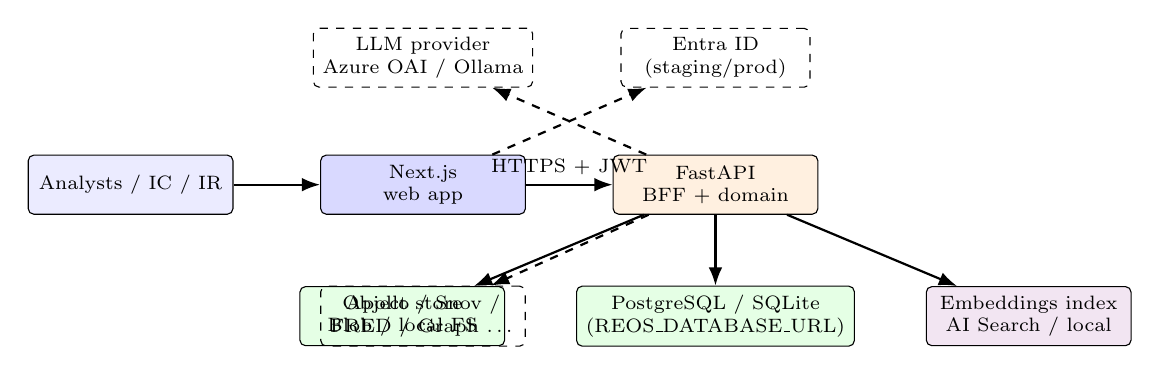
\begin{tikzpicture}[
    font=\scriptsize,
    box/.style={draw, rounded corners=2pt, align=center, minimum width=2.6cm, minimum height=0.75cm},
    ext/.style={draw, dashed, rounded corners=2pt, align=center, minimum width=2.4cm},
    line/.style={-Latex, thick},
  ]
    \node[box, fill=blue!8] (user) {Analysts / IC / IR};
    \node[box, fill=blue!15, right=1.1cm of user] (fe) {Next.js\\web app};
    \node[box, fill=orange!12, right=1.1cm of fe] (api) {FastAPI\\BFF + domain};
    \node[box, fill=green!10, below=0.9cm of api] (db) {PostgreSQL / SQLite\\(REOS\_DATABASE\_URL)};
    \node[box, fill=green!10, left=0.9cm of db] (blob) {Object store\\Blob / local FS};
    \node[box, fill=violet!10, right=0.9cm of db] (idx) {Embeddings index\\AI Search / local};
    \node[ext, above=0.85cm of api] (idp) {Entra ID\\(staging/prod)};
    \node[ext, above=0.85cm of fe] (llm) {LLM provider\\Azure OAI / Ollama};
    \node[ext, below=0.9cm of fe] (vendors) {Apollo / Snov /\\FRED / Graph \ldots};

    \draw[line] (user) -- (fe);
    \draw[line] (fe) -- node[above, sloped] {HTTPS + JWT} (api);
    \draw[line] (api) -- (db);
    \draw[line] (api) -- (blob);
    \draw[line] (api) -- (idx);
    \draw[line, dashed] (fe) -- (idp);
    \draw[line, dashed] (api) -- (llm);
    \draw[line, dashed] (api) -- (vendors);
  \end{tikzpicture}

  \vspace{0.4em}
  \footnotesize External calls exit only from API tier; browser holds no vendor keys.
\end{frame}

\begin{frame}{Trust boundaries}
  \small
  \begin{itemize}
    \item \textbf{Browser}: presentation, form validation only; zero integration secrets.
    \item \textbf{API}: authentication, RBAC, input validation, outbound connector policy, audit emit.
    \item \textbf{Workers} (target): bounded identity (managed ID), dequeue, idempotent handlers, DLQ.
    \item \textbf{Data}: row-level tenancy hooks reserved; secrets in Key Vault / env; encryption in transit everywhere.
  \end{itemize}
\end{frame}

%------------------------------------------------------------------
\section{Core workflows}

\begin{frame}{Deal and document read/write path}
  \centering
  \begin{tikzpicture}[
    font=\scriptsize,
    step/.style={draw, rounded corners=2pt, align=center, inner sep=4pt},
    arrow/.style={-Latex, thick},
  ]
    \node[step, fill=blue!10] (a) {Create / patch deal};
    \node[step, fill=blue!10, right=1.5cm of a] (b) {Stage events / checklist};
    \node[step, fill=orange!10, right=1.5cm of b] (c) {Upload doc};
    \node[step, fill=orange!20, below=0.85cm of c] (d) {Parse / OCR / chunk};
    \node[step, fill=violet!10, left=1.5cm of d] (e) {Embed + index};
    \node[step, fill=green!12, left=1.5cm of e] (f) {Link to deal + audit};

    \draw[arrow] (a) -- (b);
    \draw[arrow] (b) -- (c);
    \draw[arrow] (c) -- (d);
    \draw[arrow] (d) -- (e);
    \draw[arrow] (e) -- (f);
  \end{tikzpicture}

  \vspace{0.6em}
  \raggedright
  \footnotesize
  Transactional truth stays relational; vectors are derived and rebuildable from stored documents.
\end{frame}

\begin{frame}{RAG query path (grounded answers)}
  \centering
  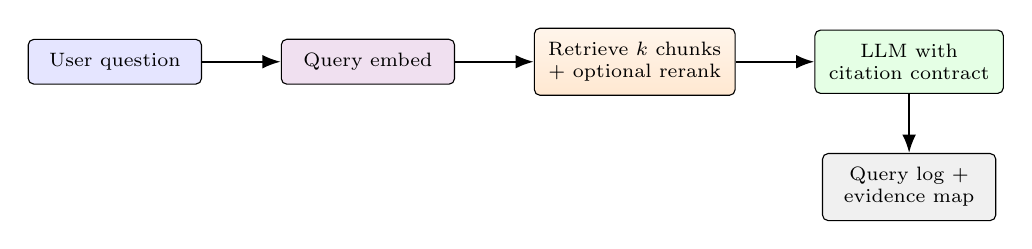
\begin{tikzpicture}[
    font=\scriptsize,
    box/.style={draw, rounded corners=2pt, align=center, minimum width=2.2cm, inner sep=5pt},
    arr/.style={-Latex, thick},
  ]
    \node[box, fill=blue!10] (q) {User question};
    \node[box, fill=violet!12, right=1cm of q] (emb) {Query embed};
    \node[box, top color=orange!8, bottom color=orange!18, right=1cm of emb] (ret) {Retrieve $k$ chunks\\+ optional rerank};
    \node[box, fill=green!10, right=1cm of ret] (llm) {LLM with\\citation contract};
    \node[box, fill=gray!12, below=0.75cm of llm] (log) {Query log +\\evidence map};

    \draw[arr] (q) -- (emb);
    \draw[arr] (emb) -- (ret);
    \draw[arr] (ret) -- (llm);
    \draw[arr] (llm) -- (log);
  \end{tikzpicture}

  \vspace{0.5em}
  \raggedright
  \small
  \begin{itemize}
    \item Responses are constrained to retrieved context; unsupported claims flagged for human review.
    \item Provider switch (Ollama $\leftrightarrow$ Azure OpenAI) is configuration, not a fork.
  \end{itemize}
\end{frame}

\begin{frame}{Integration adapter pattern (proposed norm)}
  \small
  \begin{enumerate}
    \item \textbf{Catalog entry}: capability, auth type, required env, rate-limit class, data classification.
    \item \textbf{Connector module}: single outbound client; timeouts; retries with jitter; structured errors.
    \item \textbf{Cache layer}: vendor response hashing; TTL by sensitivity; no PII in client-side caches.
    \item \textbf{Audit}: fetch metadata (vendor, deal id, correlation id) stored for reconciliation.
    \item \textbf{Feature flags}: demo mode, per-tenant enablement, kill switch.
  \end{enumerate}
\end{frame}

%------------------------------------------------------------------
\section{Challenges and how we address them}

\begin{frame}{Project challenges $\rightarrow$ approach}
  \tiny
  \begin{tabular}{p{3.35cm}p{4.15cm}p{5.5cm}}
    \textbf{Challenge} & \textbf{Why it hurts} & \textbf{Approach} \\
    \hline
    Data scattered (email, drives, CRM) & Slow IC, inconsistent numbers & Single deal graph + ingestion adapters; email as \textbf{signal} not SoT \\
    Model hallucination / overconfidence & Credibility loss, legal exposure & Retrieval-grounded answers; schema outputs; human override KPI \\
    OCR / doc variance & Missed covenants & Confidence gating; verifier queue; parser versioning + replay \\
    Tenancy and IAM complexity & Cross-tenant risk & App RBAC now; RLS on Postgres target; Entra claim mapping in staging \\
    Vendor sprawl and cost & Fragile demos & Integration catalog, caching, circuit breakers, entitlement docs \\
    Async scale-up & API timeouts & Queue + workers; idempotent jobs; DLQ and admin replay \\
    Scope creep (``AI everywhere'') & No ship & One \textbf{golden pipeline} per phase; MoSCoW in backlog \\
    Legacy spreadsheet habit & Low adoption & Import paths + parity reports until cutover criteria met \\
  \end{tabular}
\end{frame}

%------------------------------------------------------------------
\section{Objectives, priorities, and deliverables}

\begin{frame}{Actionable objectives (measurable)}
  \small
  \begin{enumerate}\itemsep4pt
    \item \textbf{O1}: Production database on Postgres with automated backups and documented restore ($\leq$ 1 h RPO target in contract).
    \item \textbf{O2}: P95 API read latency under agreed threshold on reference workload; document ingestion \textbf{async} with visible job status.
    \item \textbf{O3}: 100\% of integration connectors behind server auth; zero third-party keys in frontend bundle (verified by CI scan).
    \item \textbf{O4}: RAG evaluation set (faithfulness / citation coverage) run per release on staging before prod promote.
    \item \textbf{O5}: Decision-surface metrics exposed: median time in diligence, IC dwell, analyst hours estimate (even if v1 is heuristic).
  \end{enumerate}
\end{frame}

\begin{frame}{Priorities (execution order)}
  \centering
  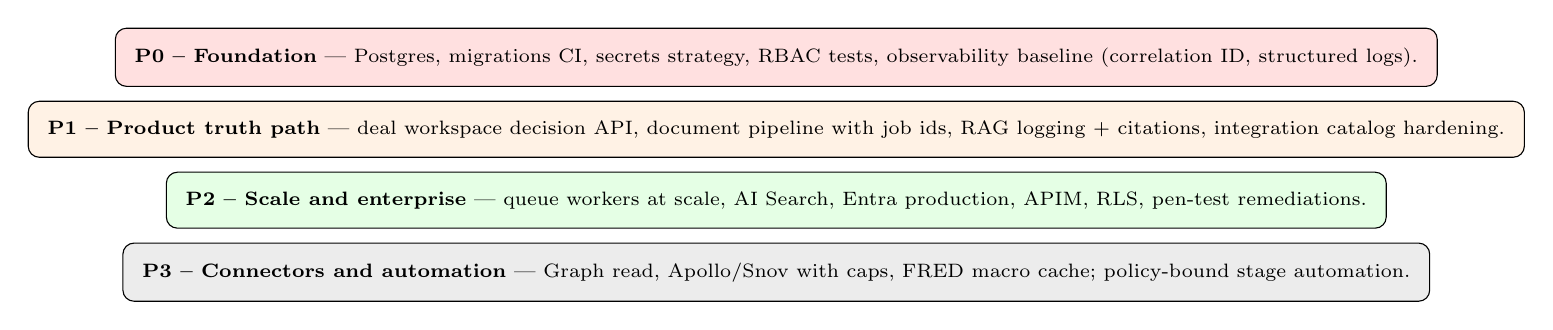
\begin{tikzpicture}[
    font=\scriptsize,
    pri/.style={draw, rounded corners=4pt, align=left, inner sep=7pt, minimum width=10.6cm},
  ]
    \node[pri, fill=red!12] (p0) {\textbf{P0 -- Foundation} --- Postgres, migrations CI, secrets strategy, RBAC tests, observability baseline (correlation ID, structured logs).};
    \node[pri, fill=orange!10, below=5pt of p0] (p1) {\textbf{P1 -- Product truth path} --- deal workspace decision API, document pipeline with job ids, RAG logging + citations, integration catalog hardening.};
    \node[pri, fill=green!10, below=5pt of p1] (p2) {\textbf{P2 -- Scale and enterprise} --- queue workers at scale, AI Search, Entra production, APIM, RLS, pen-test remediations.};
    \node[pri, fill=gray!15, below=5pt of p2] (p3) {\textbf{P3 -- Connectors and automation} --- Graph read, Apollo/Snov with caps, FRED macro cache; policy-bound stage automation.};
  \end{tikzpicture}
\end{frame}

\begin{frame}{Deliverables and representative tasks}
  \tiny
  \begin{tabular}{p{2.45cm}p{4.7cm}p{5.8cm}}
    \textbf{Deliverable} & \textbf{Outcome} & \textbf{Tasks (samples)} \\
    \hline
    D1: Data plane & HA Postgres, backups & Schema migrate; PITR; connection pooling; staging data policy \\
    D2: Identity & Entra in staging/prod & App registration; group$\rightarrow$role map; JWT middleware tests \\
    D3: Document jobs & Async OCR/embed & Queue abstraction; worker container; DLQ; status API \\
    D4: RAG enterprise & Grounded Q\&A & Azure OAI + AI Search wiring; eval harness; red-team prompts \\
    D5: Integrations & Safe vendor use & Connector modules; rate limits; audit rows; demo vs prod keys \\
    D6: Observability & Operational trust & Dashboards: queue lag, error budget, model spend caps \\
    D7: Security hardening & Contract sign-off & SAST/DAST; dep audit; OWASP ASVS subset; IR playbook \\
  \end{tabular}

  \vspace{0.35em}
  \normalsize
  Sprint planning maps tasks to \textbf{one} deliverable owner; no orphan work without acceptance criteria.
\end{frame}

\begin{frame}{Milestone map (aligns to contract phases)}
  \small
  \begin{enumerate}\itemsep3pt
    \item \textbf{M1}: Core hardening shipped---Postgres, CI gates, security baseline, runbook draft.
    \item \textbf{M2}: Async document path with observable SLI + replay tool.
    \item \textbf{M3}: Enterprise AI path in staging with eval gate before production.
    \item \textbf{M4}: First production connector family (e.g.\ macro + one enrichment) with entitlement memo.
    \item \textbf{M5}: Production go-live checklist signed (backup test, pen-test deltas, hypercare window).
  \end{enumerate}
\end{frame}

%------------------------------------------------------------------
\section{Security and governance}

\begin{frame}{Security controls (contract-grade checklist)}
  \small
  \begin{columns}[T]
    \begin{column}{0.48\textwidth}
      \textbf{Identity}
      \begin{itemize}\itemsep2pt
        \item Server-side JWT validation; role claims from Entra mapping
        \item No long-lived embed tokens in SPA storage for vendor APIs
      \end{itemize}
      \textbf{Data}
      \begin{itemize}\itemsep2pt
        \item Postgres Row Level Security (target) + app RBAC
        \item Blob SAS or managed identity; virus scan step (target)
      \end{itemize}
    \end{column}
    \begin{column}{0.48\textwidth}
      \textbf{AI safety}
      \begin{itemize}\itemsep2pt
        \item Tool allowlists; schema validation on model outputs
        \item Prompt injection mitigations: system policy, retrieval boundaries
      \end{itemize}
      \textbf{Operations}
      \begin{itemize}\itemsep2pt
        \item Structured logs + correlation ID end-to-end
        \item Override metrics for automation suggestions
      \end{itemize}
    \end{column}
  \end{columns}
\end{frame}

\begin{frame}{Automation governance}
  \small
  \begin{itemize}
    \item \textbf{Assistive} default: suggestions only; human confirms stage moves and outbound email.
    \item \textbf{Autonomous} (later): policy DSL per org---which transitions, which templates, which mailboxes.
    \item \textbf{Evidence}: every automated state change references artifact ids or rule version.
  \end{itemize}
\end{frame}

%------------------------------------------------------------------
\section{Deployment and evolution}

\begin{frame}{Environment progression}
  \centering
  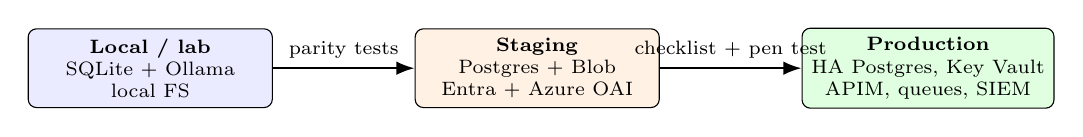
\begin{tikzpicture}[
    font=\scriptsize,
    env/.style={draw, rounded corners=3pt, align=center, minimum width=3.1cm, minimum height=1cm},
    ar/.style={-Latex, thick},
  ]
    \node[env, fill=blue!8] (l) {\textbf{Local / lab}\\SQLite + Ollama\\local FS};
    \node[env, fill=orange!10, right=1.8cm of l] (s) {\textbf{Staging}\\Postgres + Blob\\Entra + Azure OAI};
    \node[env, fill=green!12, right=1.8cm of s] (p) {\textbf{Production}\\HA Postgres, Key Vault\\APIM, queues, SIEM};

    \draw[ar] (l) -- node[above]{parity tests} (s);
    \draw[ar] (s) -- node[above]{checklist + pen test} (p);
  \end{tikzpicture}

  \vspace{0.6em}
  \raggedright
  \small
  Same container images; differences are env contract and scale-out (workers, replicas, Redis optional).
\end{frame}

\begin{frame}{Non-functional targets (proposal)}
  \small
  \begin{tabular}{ll}
    \textbf{Availability} & API 99.9\% with multi-AZ Postgres and stateless API \\
    \textbf{Latency} & P95 read $<$ 300 ms (uncached); ingestion async \\
    \textbf{Durability} & Blob versioning + DB PITR \\
    \textbf{Scale-out} & Stateless API; worker pool for OCR/embed; back-pressure on queues \\
    \textbf{Compliance path} & SOC2-oriented logging, access reviews, DPA with cloud vendors \\
  \end{tabular}
\end{frame}

%------------------------------------------------------------------
\section{Delivery plan and risks}

\begin{frame}{Phased delivery (summary)}
  \small
  Aligns with \textbf{P0--P3} and deliverables \textbf{D1--D7}: foundation first, then truth path, then enterprise scale, then connector depth. Detailed tasks live in the sprint backlog and runbooks; this deck is the \textbf{governance spine} for acceptance.
  \vspace{0.5em}
  \begin{itemize}\itemsep2pt
    \item Phase tie-breaker: if slipping, cut \textbf{connector breadth}, never cut \textbf{audit}, \textbf{RBAC}, or \textbf{backup}.
  \end{itemize}
\end{frame}

\begin{frame}{Risk register (excerpt)}
  \tiny
  \begin{tabular}{p{3.8cm}p{4.2cm}p{4.5cm}}
    \textbf{Risk} & \textbf{Impact} & \textbf{Mitigation} \\
    \hline
    Model drift / hallucination & Wrong IC narrative & Retrieval-only answers; eval set; human override KPI \\
    Vendor API instability & Broken comps or enrichment & Circuit breaker; cached fallbacks; feature flags \\
    Tenancy bugs & Cross-customer leak & RLS + integration tests + audit \\
    OCR quality & Missed clauses & Confidence scores; human verification queue \\
    Scope creep on ``automation'' & Never ships & One golden pipeline per quarter; timeboxed phases \\
  \end{tabular}
\end{frame}

\begin{frame}{Why this architecture wins the build}
  \small
  \begin{itemize}
    \item \textbf{Boring core}: relational source of truth, explicit workflow state, boring object storage.
    \item \textbf{Clear seams}: BFF owns policy; workers own latency; connectors are replaceable.
    \item \textbf{Measurable}: time-in-stage, ingestion latency, override rate, retrieval precision@$k$.
    \item \textbf{Defensible}: audit trail, human gates, no magic autonomy on capital.
  \end{itemize}
\end{frame}

\begin{frame}
  \centering
  \Large Technical Q\&A
\end{frame}

\appendix

\section*{Appendix}

\begin{frame}{HTTP surface (contract)}
  \small
  \begin{itemize}
    \item FastAPI exposes versioned REST under a single app; auth via Bearer token (local) or Entra-validated JWT (target enterprise).
    \item Integration catalog: \texttt{/integrations/catalog} (read), toggle and prefs for operator demos.
    \item Domain: deals, CRM, documents, diligence, investor pipeline, dashboard aggregates, AI query logs.
    \item OpenAPI schema ships with the codebase; can export for consumer SDK generation in Phase 1.
  \end{itemize}
\end{frame}

\begin{frame}{Document ingestion sequence (target async)}
  \centering
  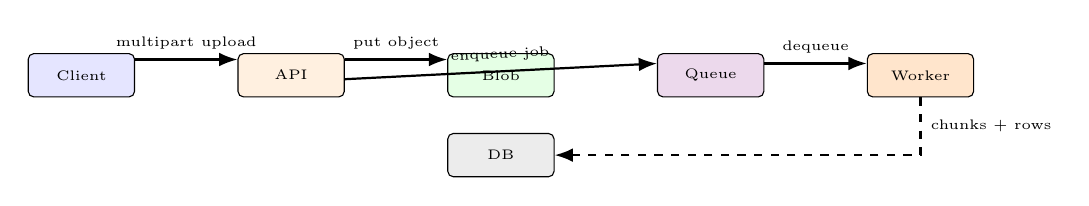
\begin{tikzpicture}[
    font=\tiny,
    actor/.style={rectangle, draw, rounded corners=2pt, minimum width=1.35cm, minimum height=0.55cm, align=center},
    msg/.style={-Latex, thick},
  ]
    \node[actor, fill=blue!10] (cl) {Client};
    \node[actor, fill=orange!12, right=1.3cm of cl] (api) {API};
    \node[actor, fill=green!10, right=1.3cm of api] (blob) {Blob};
    \node[actor, fill=violet!15, right=1.3cm of blob] (q) {Queue};
    \node[actor, fill=orange!20, right=1.3cm of q] (wk) {Worker};
    \node[actor, fill=gray!15, below=0.45cm of blob] (db) {DB};

    \draw[msg] ($(cl.east)+(0,0.2)$) -- node[above]{multipart upload} ($(api.west)+(0,0.2)$);
    \draw[msg] ($(api.east)+(0,0.2)$) -- node[above]{put object} ($(blob.west)+(0,0.2)$);
    \draw[msg] ($(api.east)+(0,-0.05)$) -- node[above, sloped]{enqueue job} ($(q.west)+(0,0.15)$);
    \draw[msg] ($(q.east)+(0,0.15)$) -- node[above]{dequeue} ($(wk.west)+(0,0.15)$);
    \draw[msg, dashed] ($(wk.south)$) |- node[near start, right]{chunks + rows} ($(db.east)$);
  \end{tikzpicture}

  \vspace{0.5em}
  \raggedright
  \footnotesize
  Today: parts run in-process. Production: API returns \texttt{202} + job id; worker idempotency key = (document\_id, parser\_version).
\end{frame}

\begin{frame}{Test and quality gates}
  \small
  \begin{itemize}
    \item \textbf{Unit}: domain rules, RBAC decorators, schema validation.
    \item \textbf{API integration}: pytest + TestClient; fresh DB per test module where needed.
    \item \textbf{Contract}: optional schemathesis against OpenAPI in CI (staging).
    \item \textbf{Load}: k6 or Locust on read-heavy paths before GA.
    \item \textbf{Security}: OWASP ASVS subset, dependency audit, SAST in pipeline.
  \end{itemize}
\end{frame}

\begin{frame}{Decision log (architecture)}
  \small
  \begin{tabular}{p{3.3cm}p{8.2cm}}
    \textbf{Monolith BFF first} & Faster iteration; extract workers when queue depth or OCR CPU demands it. \\
    \textbf{Postgres not mandatory on day one} & Code path exists; cutover is env-driven and migration-backed. \\
    \textbf{Vectors are derived} & Rebuild index from source blobs; avoids split-brain with PDF truth. \\
    \textbf{Human gates stay in domain} & Automation modes are policy, not model temperature. \\
  \end{tabular}
\end{frame}

\end{document}

